\documentclass[1p]{elsarticle_modified}
%\bibliographystyle{elsarticle-num}

%\usepackage[colorlinks]{hyperref}
%\usepackage{abbrmath_seonhwa} %\Abb, \Ascr, \Acal ,\Abf, \Afrak
\usepackage{amsfonts}
\usepackage{amssymb}
\usepackage{amsmath}
\usepackage{amsthm}
\usepackage{scalefnt}
\usepackage{amsbsy}
\usepackage{kotex}
\usepackage{caption}
\usepackage{subfig}
\usepackage{color}
\usepackage{graphicx}
\usepackage{xcolor} %% white, black, red, green, blue, cyan, magenta, yellow
\usepackage{float}
\usepackage{setspace}
\usepackage{hyperref}

\usepackage{tikz}
\usetikzlibrary{arrows}

\usepackage{multirow}
\usepackage{array} % fixed length table
\usepackage{hhline}

%%%%%%%%%%%%%%%%%%%%%
\makeatletter
\renewcommand*\env@matrix[1][\arraystretch]{%
	\edef\arraystretch{#1}%
	\hskip -\arraycolsep
	\let\@ifnextchar\new@ifnextchar
	\array{*\c@MaxMatrixCols c}}
\makeatother %https://tex.stackexchange.com/questions/14071/how-can-i-increase-the-line-spacing-in-a-matrix
%%%%%%%%%%%%%%%

\usepackage[normalem]{ulem}

\newcommand{\msout}[1]{\ifmmode\text{\sout{\ensuremath{#1}}}\else\sout{#1}\fi}
%SOURCE: \msout is \stkout macro in https://tex.stackexchange.com/questions/20609/strikeout-in-math-mode

\newcommand{\cancel}[1]{
	\ifmmode
	{\color{red}\msout{#1}}
	\else
	{\color{red}\sout{#1}}
	\fi
}

\newcommand{\add}[1]{
	{\color{blue}\uwave{#1}}
}

\newcommand{\replace}[2]{
	\ifmmode
	{\color{red}\msout{#1}}{\color{blue}\uwave{#2}}
	\else
	{\color{red}\sout{#1}}{\color{blue}\uwave{#2}}
	\fi
}

\newcommand{\Sol}{\mathcal{S}} %segment
\newcommand{\D}{D} %diagram
\newcommand{\A}{\mathcal{A}} %arc


%%%%%%%%%%%%%%%%%%%%%%%%%%%%%5 test

\def\sl{\operatorname{\textup{SL}}(2,\Cbb)}
\def\psl{\operatorname{\textup{PSL}}(2,\Cbb)}
\def\quan{\mkern 1mu \triangleright \mkern 1mu}

\theoremstyle{definition}
\newtheorem{thm}{Theorem}[section]
\newtheorem{prop}[thm]{Proposition}
\newtheorem{lem}[thm]{Lemma}
\newtheorem{ques}[thm]{Question}
\newtheorem{cor}[thm]{Corollary}
\newtheorem{defn}[thm]{Definition}
\newtheorem{exam}[thm]{Example}
\newtheorem{rmk}[thm]{Remark}
\newtheorem{alg}[thm]{Algorithm}

\newcommand{\I}{\sqrt{-1}}
\begin{document}

%\begin{frontmatter}
%
%\title{Boundary parabolic representations of knots up to 8 crossings}
%
%%% Group authors per affiliation:
%\author{Yunhi Cho} 
%\address{Department of Mathematics, University of Seoul, Seoul, Korea}
%\ead{yhcho@uos.ac.kr}
%
%
%\author{Seonhwa Kim} %\fnref{s_kim}}
%\address{Center for Geometry and Physics, Institute for Basic Science, Pohang, 37673, Korea}
%\ead{ryeona17@ibs.re.kr}
%
%\author{Hyuk Kim}
%\address{Department of Mathematical Sciences, Seoul National University, Seoul 08826, Korea}
%\ead{hyukkim@snu.ac.kr}
%
%\author{Seokbeom Yoon}
%\address{Department of Mathematical Sciences, Seoul National University, Seoul, 08826,  Korea}
%\ead{sbyoon15@snu.ac.kr}
%
%\begin{abstract}
%We find all boundary parabolic representation of knots up to 8 crossings.
%
%\end{abstract}
%\begin{keyword}
%    \MSC[2010] 57M25 
%\end{keyword}
%
%\end{frontmatter}

%\linenumbers
%\tableofcontents
%
\newcommand\colored[1]{\textcolor{white}{\rule[-0.35ex]{0.8em}{1.4ex}}\kern-0.8em\color{red} #1}%
%\newcommand\colored[1]{\textcolor{white}{ #1}\kern-2.17ex	\textcolor{white}{ #1}\kern-1.81ex	\textcolor{white}{ #1}\kern-2.15ex\color{red}#1	}

{\Large $\underline{11a_{280}~(K11a_{280})}$}

\setlength{\tabcolsep}{10pt}
\renewcommand{\arraystretch}{1.6}
\vspace{1cm}\begin{tabular}{m{100pt}>{\centering\arraybackslash}m{274pt}}
\multirow{5}{120pt}{
	\centering
	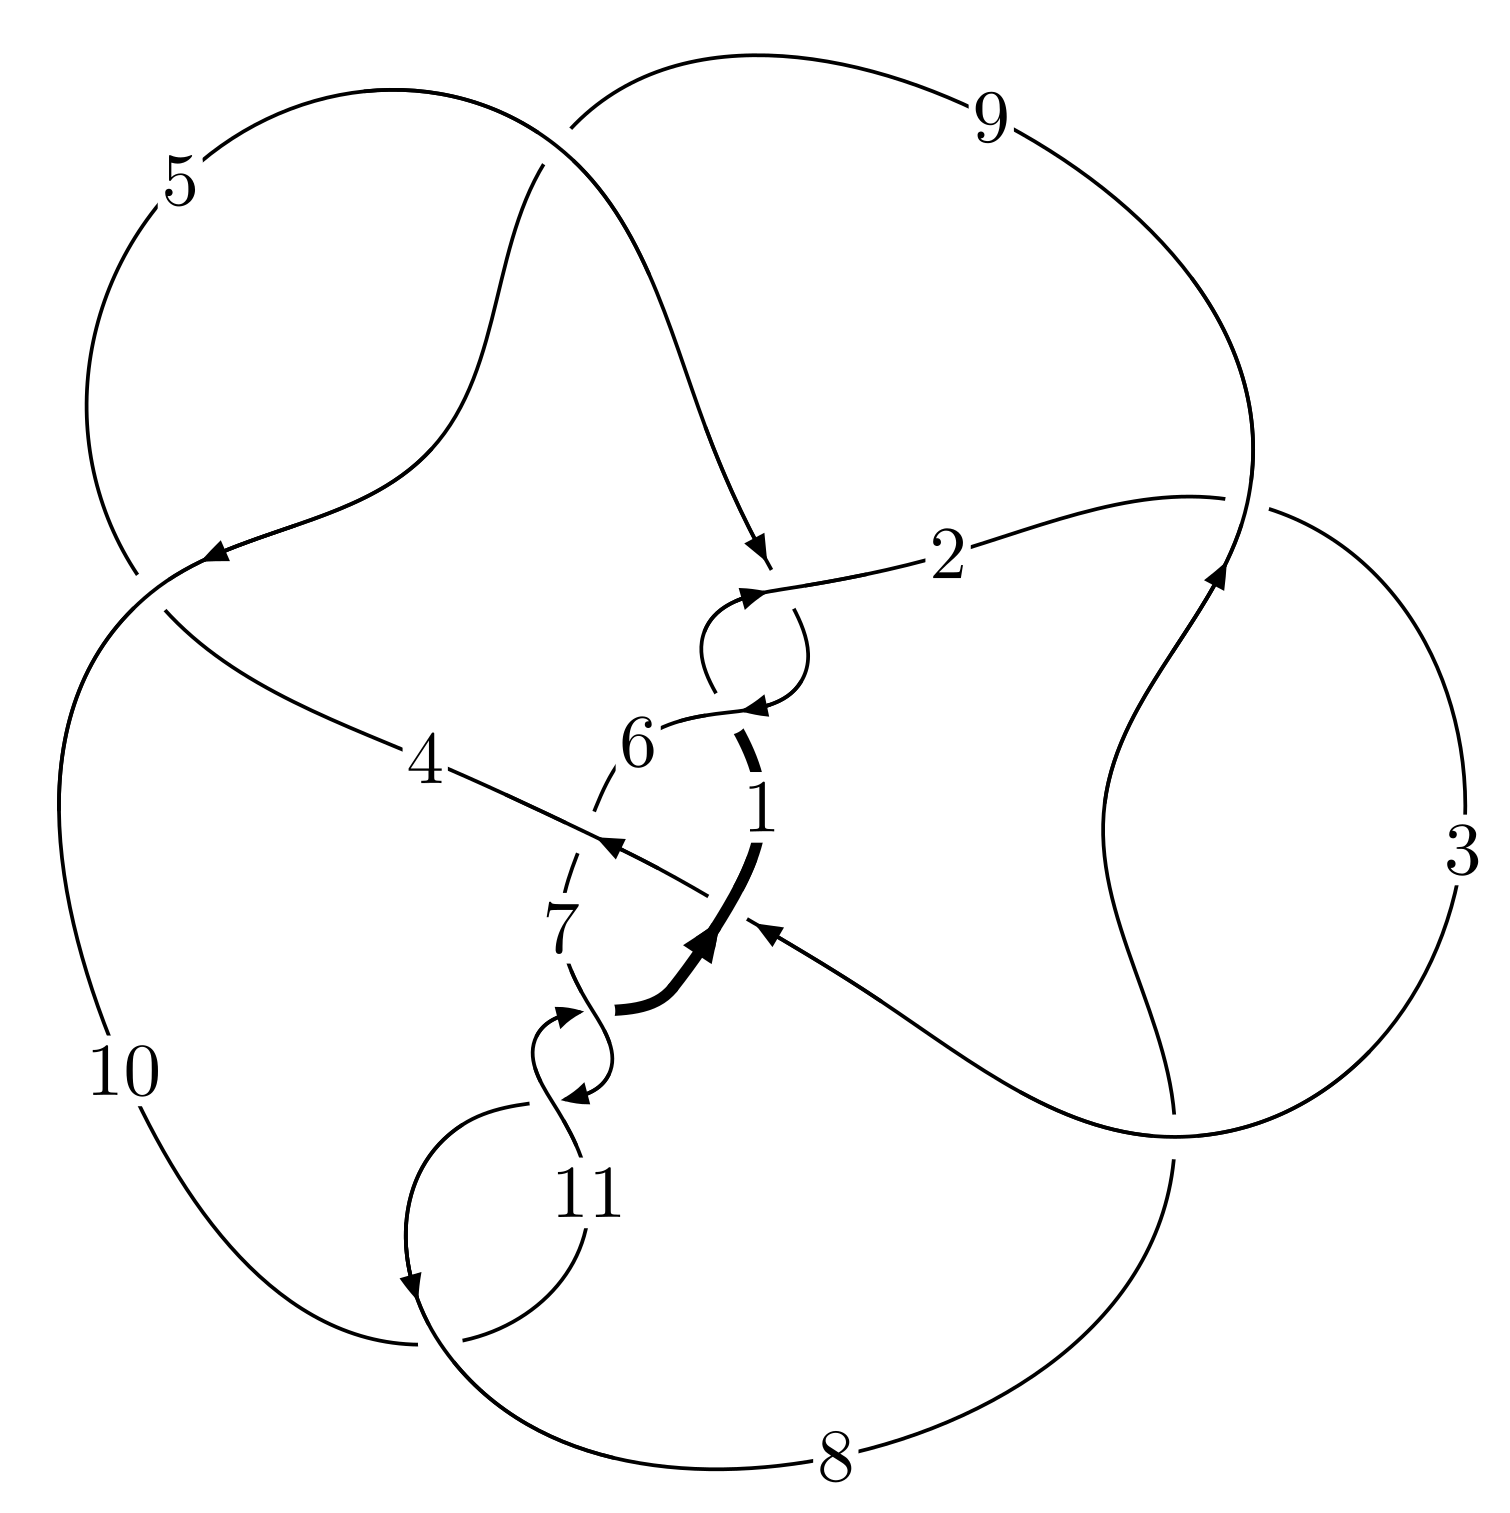
\includegraphics[width=112pt]{../../../GIT/diagram.site/Diagrams/png/529_11a_280.png}\\
\ \ \ A knot diagram\footnotemark}&
\allowdisplaybreaks
\textbf{Linearized knot diagam} \\
\cline{2-2}
 &
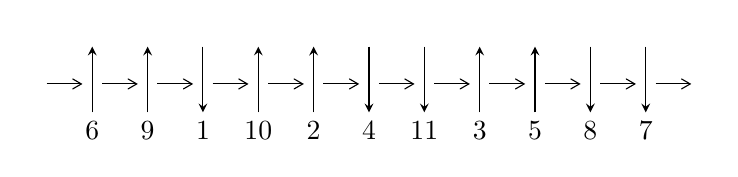
\begin{tikzpicture}[x=20pt, y=17pt]
	% nodes
	\node (C0) at (0, 0) {};
	\node (C1) at (1, 0) {};
	\node (C1U) at (1, +1) {};
	\node (C1D) at (1, -1) {6};

	\node (C2) at (2, 0) {};
	\node (C2U) at (2, +1) {};
	\node (C2D) at (2, -1) {9};

	\node (C3) at (3, 0) {};
	\node (C3U) at (3, +1) {};
	\node (C3D) at (3, -1) {1};

	\node (C4) at (4, 0) {};
	\node (C4U) at (4, +1) {};
	\node (C4D) at (4, -1) {10};

	\node (C5) at (5, 0) {};
	\node (C5U) at (5, +1) {};
	\node (C5D) at (5, -1) {2};

	\node (C6) at (6, 0) {};
	\node (C6U) at (6, +1) {};
	\node (C6D) at (6, -1) {4};

	\node (C7) at (7, 0) {};
	\node (C7U) at (7, +1) {};
	\node (C7D) at (7, -1) {11};

	\node (C8) at (8, 0) {};
	\node (C8U) at (8, +1) {};
	\node (C8D) at (8, -1) {3};

	\node (C9) at (9, 0) {};
	\node (C9U) at (9, +1) {};
	\node (C9D) at (9, -1) {5};

	\node (C10) at (10, 0) {};
	\node (C10U) at (10, +1) {};
	\node (C10D) at (10, -1) {8};

	\node (C11) at (11, 0) {};
	\node (C11U) at (11, +1) {};
	\node (C11D) at (11, -1) {7};
	\node (C12) at (12, 0) {};

	% arrows
	\draw[->,>={angle 60}]
	(C0) edge (C1) (C1) edge (C2) (C2) edge (C3) (C3) edge (C4) (C4) edge (C5) (C5) edge (C6) (C6) edge (C7) (C7) edge (C8) (C8) edge (C9) (C9) edge (C10) (C10) edge (C11) (C11) edge (C12) ;	\draw[->,>=stealth]
	(C1D) edge (C1U) (C2D) edge (C2U) (C3U) edge (C3D) (C4D) edge (C4U) (C5D) edge (C5U) (C6U) edge (C6D) (C7U) edge (C7D) (C8D) edge (C8U) (C9D) edge (C9U) (C10U) edge (C10D) (C11U) edge (C11D) ;
	\end{tikzpicture} \\
\hhline{~~} \\& 
\textbf{Solving Sequence} \\ \cline{2-2} 
 &
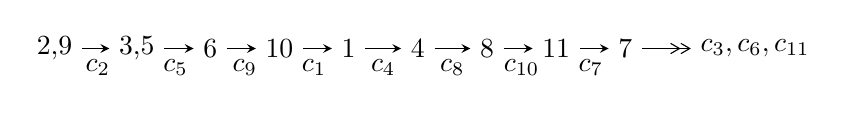
\begin{tikzpicture}[x=25pt, y=7pt]
	% node
	\node (A0) at (-1/8, 0) {2,9};
	\node (A1) at (17/16, 0) {3,5};
	\node (A2) at (17/8, 0) {6};
	\node (A3) at (25/8, 0) {10};
	\node (A4) at (33/8, 0) {1};
	\node (A5) at (41/8, 0) {4};
	\node (A6) at (49/8, 0) {8};
	\node (A7) at (57/8, 0) {11};
	\node (A8) at (65/8, 0) {7};
	\node (C1) at (1/2, -1) {$c_{2}$};
	\node (C2) at (13/8, -1) {$c_{5}$};
	\node (C3) at (21/8, -1) {$c_{9}$};
	\node (C4) at (29/8, -1) {$c_{1}$};
	\node (C5) at (37/8, -1) {$c_{4}$};
	\node (C6) at (45/8, -1) {$c_{8}$};
	\node (C7) at (53/8, -1) {$c_{10}$};
	\node (C8) at (61/8, -1) {$c_{7}$};
	\node (A9) at (10, 0) {$c_{3},c_{6},c_{11}$};

	% edge
	\draw[->,>=stealth]	
	(A0) edge (A1) (A1) edge (A2) (A2) edge (A3) (A3) edge (A4) (A4) edge (A5) (A5) edge (A6) (A6) edge (A7) (A7) edge (A8) ;
	\draw[->>,>={angle 60}]	
	(A8) edge (A9);
\end{tikzpicture} \\ 

\end{tabular} \\

\footnotetext{
The image of knot diagram is generated by the software ``\textbf{Draw programme}" developed by Andrew Bartholomew(\url{http://www.layer8.co.uk/maths/draw/index.htm\#Running-draw}), where we modified some parts for our purpose(\url{https://github.com/CATsTAILs/LinksPainter}).
}\phantom \\ \newline 
\centering \textbf{Ideals for irreducible components\footnotemark of $X_{\text{par}}$} 
 
\begin{align*}
I^u_{1}&=\langle 
37345311 u^{21}+18480167 u^{20}+\cdots+14331796 b-87054847,\;a-1,\;u^{22}+9 u^{20}+\cdots-3 u^2+1\rangle \\
I^u_{2}&=\langle 
-2105832678 u^{17}+16757581 u^{16}+\cdots+17708562289 b-38848951730,\\
\phantom{I^u_{2}}&\phantom{= \langle  }721895222078 u^{17}-1381269075020 u^{16}+\cdots+12944959033259 a-17573961275067,\\
\phantom{I^u_{2}}&\phantom{= \langle  }u^{18}+5 u^{16}+\cdots+50 u+17\rangle \\
I^u_{3}&=\langle 
6 u^{11}+12 u^{10}+38 u^9+71 u^8+111 u^7+169 u^6+154 u^5+168 u^4+93 u^3+67 u^2+11 b+26 u+19,\;a+1,\\
\phantom{I^u_{3}}&\phantom{= \langle  }u^{12}+6 u^{10}+u^9+15 u^8+4 u^7+17 u^6+6 u^5+9 u^4+4 u^3+4 u^2+1\rangle \\
I^u_{4}&=\langle 
-1.19860\times10^{15} u^{23}+6.59553\times10^{15} u^{22}+\cdots+1.10953\times10^{17} b+2.38445\times10^{17},\\
\phantom{I^u_{4}}&\phantom{= \langle  }6.76587\times10^{19} u^{23}-7.15855\times10^{18} u^{22}+\cdots+7.49046\times10^{20} a+4.99902\times10^{21},\;u^{24}- u^{23}+\cdots-188 u+43\rangle \\
\\
\end{align*}
\raggedright * 4 irreducible components of $\dim_{\mathbb{C}}=0$, with total 76 representations.\\
\footnotetext{All coefficients of polynomials are rational numbers. But the coefficients are sometimes approximated in decimal forms when there is not enough margin.}
\newpage
\renewcommand{\arraystretch}{1}
\centering \section*{I. $I^u_{1}= \langle 3.73\times10^{7} u^{21}+1.85\times10^{7} u^{20}+\cdots+1.43\times10^{7} b-8.71\times10^{7},\;a-1,\;u^{22}+9 u^{20}+\cdots-3 u^2+1 \rangle$}
\flushleft \textbf{(i) Arc colorings}\\
\begin{tabular}{m{7pt} m{180pt} m{7pt} m{180pt} }
\flushright $a_{2}=$&$\begin{pmatrix}1\\0\end{pmatrix}$ \\
\flushright $a_{9}=$&$\begin{pmatrix}0\\u\end{pmatrix}$ \\
\flushright $a_{3}=$&$\begin{pmatrix}1\\- u^2\end{pmatrix}$ \\
\flushright $a_{5}=$&$\begin{pmatrix}1\\-2.60577 u^{21}-1.28945 u^{20}+\cdots+13.4587 u+6.07425\end{pmatrix}$ \\
\flushright $a_{6}=$&$\begin{pmatrix}-2.60577 u^{21}-1.28945 u^{20}+\cdots+13.4587 u+7.07425\\-2.60577 u^{21}-1.28945 u^{20}+\cdots+13.4587 u+6.07425\end{pmatrix}$ \\
\flushright $a_{10}=$&$\begin{pmatrix}u\\-1.28945 u^{21}-0.754726 u^{20}+\cdots+7.07425 u+2.60577\end{pmatrix}$ \\
\flushright $a_{1}=$&$\begin{pmatrix}-0.192382 u^{21}-0.424472 u^{20}+\cdots+1.45999 u+1.31709\\2.41338 u^{21}+0.864980 u^{20}+\cdots-11.9987 u-5.75715\end{pmatrix}$ \\
\flushright $a_{4}=$&$\begin{pmatrix}u^2+1\\-3.36049 u^{21}-1.72488 u^{20}+\cdots+16.0645 u+7.36370\end{pmatrix}$ \\
\flushright $a_{8}=$&$\begin{pmatrix}- u\\u^3+u\end{pmatrix}$ \\
\flushright $a_{11}=$&$\begin{pmatrix}0.435428 u^{21}+0.0330632 u^{20}+\cdots-0.289452 u-0.754726\\-1.66963 u^{21}-0.847225 u^{20}+\cdots+8.79913 u+3.39356\end{pmatrix}$ \\
\flushright $a_{7}=$&$\begin{pmatrix}0.125776 u^{21}+0.298531 u^{20}+\cdots-0.550624 u+0.520875\\-0.660480 u^{21}-0.405082 u^{20}+\cdots+5.84008 u+2.31835\end{pmatrix}$\\ \flushright $a_{7}=$&$\begin{pmatrix}0.125776 u^{21}+0.298531 u^{20}+\cdots-0.550624 u+0.520875\\-0.660480 u^{21}-0.405082 u^{20}+\cdots+5.84008 u+2.31835\end{pmatrix}$\\&\end{tabular}
\flushleft \textbf{(ii) Obstruction class $= -1$}\\~\\
\flushleft \textbf{(iii) Cusp Shapes $= -\frac{30437693}{3582949} u^{21}-\frac{22461818}{3582949} u^{20}+\cdots+\frac{186266132}{3582949} u+\frac{101532156}{3582949}$}\\~\\
\newpage\renewcommand{\arraystretch}{1}
\flushleft \textbf{(iv) u-Polynomials at the component}\newline \\
\begin{tabular}{m{50pt}|m{274pt}}
Crossings & \hspace{64pt}u-Polynomials at each crossing \\
\hline $$\begin{aligned}c_{1},c_{5}\end{aligned}$$&$\begin{aligned}
&u^{22}-14 u^{21}+\cdots-1344 u+128
\end{aligned}$\\
\hline $$\begin{aligned}c_{2},c_{4},c_{8}\\c_{9}\end{aligned}$$&$\begin{aligned}
&u^{22}+9 u^{20}+\cdots-3 u^2+1
\end{aligned}$\\
\hline $$\begin{aligned}c_{3},c_{6}\end{aligned}$$&$\begin{aligned}
&u^{22}- u^{21}+\cdots+3 u+1
\end{aligned}$\\
\hline $$\begin{aligned}c_{7},c_{10},c_{11}\end{aligned}$$&$\begin{aligned}
&u^{22}-9 u^{21}+\cdots-88 u+8
\end{aligned}$\\
\hline
\end{tabular}\\~\\
\newpage\renewcommand{\arraystretch}{1}
\flushleft \textbf{(v) Riley Polynomials at the component}\newline \\
\begin{tabular}{m{50pt}|m{274pt}}
Crossings & \hspace{64pt}Riley Polynomials at each crossing \\
\hline $$\begin{aligned}c_{1},c_{5}\end{aligned}$$&$\begin{aligned}
&y^{22}+14 y^{21}+\cdots+20480 y+16384
\end{aligned}$\\
\hline $$\begin{aligned}c_{2},c_{4},c_{8}\\c_{9}\end{aligned}$$&$\begin{aligned}
&y^{22}+18 y^{21}+\cdots-6 y+1
\end{aligned}$\\
\hline $$\begin{aligned}c_{3},c_{6}\end{aligned}$$&$\begin{aligned}
&y^{22}+5 y^{21}+\cdots+11 y+1
\end{aligned}$\\
\hline $$\begin{aligned}c_{7},c_{10},c_{11}\end{aligned}$$&$\begin{aligned}
&y^{22}+21 y^{21}+\cdots+224 y+64
\end{aligned}$\\
\hline
\end{tabular}\\~\\
\newpage\flushleft \textbf{(vi) Complex Volumes and Cusp Shapes}
$$\begin{array}{c|c|c}  
\text{Solutions to }I^u_{1}& \I (\text{vol} + \sqrt{-1}CS) & \text{Cusp shape}\\
 \hline 
\begin{aligned}
u &= \phantom{-}0.767600 + 0.519015 I \\
a &= \phantom{-}1.00000\phantom{ +0.000000I} \\
b &= -0.721664 - 0.260594 I\end{aligned}
 & \phantom{-}6.82374 - 0.02012 I & \phantom{-}7.10708 - 2.25648 I \\ \hline\begin{aligned}
u &= \phantom{-}0.767600 - 0.519015 I \\
a &= \phantom{-}1.00000\phantom{ +0.000000I} \\
b &= -0.721664 + 0.260594 I\end{aligned}
 & \phantom{-}6.82374 + 0.02012 I & \phantom{-}7.10708 + 2.25648 I \\ \hline\begin{aligned}
u &= -0.020372 + 1.119260 I \\
a &= \phantom{-}1.00000\phantom{ +0.000000I} \\
b &= -1.15684 + 1.18640 I\end{aligned}
 & -0.15255 + 1.75803 I & \phantom{-}3.02278 - 3.33932 I \\ \hline\begin{aligned}
u &= -0.020372 - 1.119260 I \\
a &= \phantom{-}1.00000\phantom{ +0.000000I} \\
b &= -1.15684 - 1.18640 I\end{aligned}
 & -0.15255 - 1.75803 I & \phantom{-}3.02278 + 3.33932 I \\ \hline\begin{aligned}
u &= -0.440574 + 0.756721 I \\
a &= \phantom{-}1.00000\phantom{ +0.000000I} \\
b &= \phantom{-}0.232862 + 1.365440 I\end{aligned}
 & \phantom{-}1.47923 - 2.31516 I & \phantom{-}0.190328 - 0.743726 I \\ \hline\begin{aligned}
u &= -0.440574 - 0.756721 I \\
a &= \phantom{-}1.00000\phantom{ +0.000000I} \\
b &= \phantom{-}0.232862 - 1.365440 I\end{aligned}
 & \phantom{-}1.47923 + 2.31516 I & \phantom{-}0.190328 + 0.743726 I \\ \hline\begin{aligned}
u &= \phantom{-}0.202451 + 1.186340 I \\
a &= \phantom{-}1.00000\phantom{ +0.000000I} \\
b &= -1.37277 - 0.52957 I\end{aligned}
 & -3.56765 + 4.49595 I & -1.80270 - 7.56758 I \\ \hline\begin{aligned}
u &= \phantom{-}0.202451 - 1.186340 I \\
a &= \phantom{-}1.00000\phantom{ +0.000000I} \\
b &= -1.37277 + 0.52957 I\end{aligned}
 & -3.56765 - 4.49595 I & -1.80270 + 7.56758 I \\ \hline\begin{aligned}
u &= -0.699025 + 0.302848 I \\
a &= \phantom{-}1.00000\phantom{ +0.000000I} \\
b &= -0.492780 - 1.057530 I\end{aligned}
 & \phantom{-}4.51267 + 4.47073 I & \phantom{-}3.53570 - 1.33986 I \\ \hline\begin{aligned}
u &= -0.699025 - 0.302848 I \\
a &= \phantom{-}1.00000\phantom{ +0.000000I} \\
b &= -0.492780 + 1.057530 I\end{aligned}
 & \phantom{-}4.51267 - 4.47073 I & \phantom{-}3.53570 + 1.33986 I\\
 \hline 
 \end{array}$$\newpage$$\begin{array}{c|c|c}  
\text{Solutions to }I^u_{1}& \I (\text{vol} + \sqrt{-1}CS) & \text{Cusp shape}\\
 \hline 
\begin{aligned}
u &= -0.375582 + 1.259580 I \\
a &= \phantom{-}1.00000\phantom{ +0.000000I} \\
b &= -1.201050 + 0.354294 I\end{aligned}
 & \phantom{-}2.08640 - 9.42284 I & \phantom{-}1.11756 + 6.83027 I \\ \hline\begin{aligned}
u &= -0.375582 - 1.259580 I \\
a &= \phantom{-}1.00000\phantom{ +0.000000I} \\
b &= -1.201050 - 0.354294 I\end{aligned}
 & \phantom{-}2.08640 + 9.42284 I & \phantom{-}1.11756 - 6.83027 I \\ \hline\begin{aligned}
u &= \phantom{-}0.408516 + 1.337620 I \\
a &= \phantom{-}1.00000\phantom{ +0.000000I} \\
b &= -0.49290 - 1.67050 I\end{aligned}
 & -8.96137 + 5.23240 I & -4.36005 - 4.78438 I \\ \hline\begin{aligned}
u &= \phantom{-}0.408516 - 1.337620 I \\
a &= \phantom{-}1.00000\phantom{ +0.000000I} \\
b &= -0.49290 + 1.67050 I\end{aligned}
 & -8.96137 - 5.23240 I & -4.36005 + 4.78438 I \\ \hline\begin{aligned}
u &= -0.408610 + 0.359797 I \\
a &= \phantom{-}1.00000\phantom{ +0.000000I} \\
b &= -0.421704 + 0.476349 I\end{aligned}
 & \phantom{-}0.735294 - 0.892872 I & \phantom{-}5.94617 + 4.93873 I \\ \hline\begin{aligned}
u &= -0.408610 - 0.359797 I \\
a &= \phantom{-}1.00000\phantom{ +0.000000I} \\
b &= -0.421704 - 0.476349 I\end{aligned}
 & \phantom{-}0.735294 + 0.892872 I & \phantom{-}5.94617 - 4.93873 I \\ \hline\begin{aligned}
u &= \phantom{-}0.468145 + 0.007430 I \\
a &= \phantom{-}1.00000\phantom{ +0.000000I} \\
b &= -0.420259 - 0.946349 I\end{aligned}
 & -0.61105 + 2.59129 I & \phantom{-}5.45931 - 3.44339 I \\ \hline\begin{aligned}
u &= \phantom{-}0.468145 - 0.007430 I \\
a &= \phantom{-}1.00000\phantom{ +0.000000I} \\
b &= -0.420259 + 0.946349 I\end{aligned}
 & -0.61105 - 2.59129 I & \phantom{-}5.45931 + 3.44339 I \\ \hline\begin{aligned}
u &= -0.50268 + 1.47148 I \\
a &= \phantom{-}1.00000\phantom{ +0.000000I} \\
b &= -0.48500 + 1.56416 I\end{aligned}
 & -10.0188 - 10.9083 I & -4.45406 + 7.18292 I \\ \hline\begin{aligned}
u &= -0.50268 - 1.47148 I \\
a &= \phantom{-}1.00000\phantom{ +0.000000I} \\
b &= -0.48500 - 1.56416 I\end{aligned}
 & -10.0188 + 10.9083 I & -4.45406 - 7.18292 I\\
 \hline 
 \end{array}$$\newpage$$\begin{array}{c|c|c}  
\text{Solutions to }I^u_{1}& \I (\text{vol} + \sqrt{-1}CS) & \text{Cusp shape}\\
 \hline 
\begin{aligned}
u &= \phantom{-}0.60013 + 1.53489 I \\
a &= \phantom{-}1.00000\phantom{ +0.000000I} \\
b &= -0.46789 - 1.52014 I\end{aligned}
 & -3.8405 + 15.3110 I & -0.76212 - 7.48531 I \\ \hline\begin{aligned}
u &= \phantom{-}0.60013 - 1.53489 I \\
a &= \phantom{-}1.00000\phantom{ +0.000000I} \\
b &= -0.46789 + 1.52014 I\end{aligned}
 & -3.8405 - 15.3110 I & -0.76212 + 7.48531 I\\
 \hline 
 \end{array}$$\newpage\newpage\renewcommand{\arraystretch}{1}
\centering \section*{II. $I^u_{2}= \langle -2.11\times10^{9} u^{17}+1.68\times10^{7} u^{16}+\cdots+1.77\times10^{10} b-3.88\times10^{10},\;7.22\times10^{11} u^{17}-1.38\times10^{12} u^{16}+\cdots+1.29\times10^{13} a-1.76\times10^{13},\;u^{18}+5 u^{16}+\cdots+50 u+17 \rangle$}
\flushleft \textbf{(i) Arc colorings}\\
\begin{tabular}{m{7pt} m{180pt} m{7pt} m{180pt} }
\flushright $a_{2}=$&$\begin{pmatrix}1\\0\end{pmatrix}$ \\
\flushright $a_{9}=$&$\begin{pmatrix}0\\u\end{pmatrix}$ \\
\flushright $a_{3}=$&$\begin{pmatrix}1\\- u^2\end{pmatrix}$ \\
\flushright $a_{5}=$&$\begin{pmatrix}-0.0557665 u^{17}+0.106703 u^{16}+\cdots+0.722131 u+1.35759\\0.118916 u^{17}-0.000946298 u^{16}+\cdots+6.12291 u+2.19379\end{pmatrix}$ \\
\flushright $a_{6}=$&$\begin{pmatrix}0.0631496 u^{17}+0.105757 u^{16}+\cdots+6.84504 u+3.55139\\0.118916 u^{17}-0.000946298 u^{16}+\cdots+6.12291 u+2.19379\end{pmatrix}$ \\
\flushright $a_{10}=$&$\begin{pmatrix}0.130783 u^{17}-0.0146315 u^{16}+\cdots+6.70179 u+1.56799\\0.0513201 u^{17}-0.0379460 u^{16}+\cdots+0.584746 u-1.26324\end{pmatrix}$ \\
\flushright $a_{1}=$&$\begin{pmatrix}0.188268 u^{17}-0.0221695 u^{16}+\cdots+11.5572 u+3.70897\\0.113960 u^{17}-0.0734896 u^{16}+\cdots+2.32962 u-0.591198\end{pmatrix}$ \\
\flushright $a_{4}=$&$\begin{pmatrix}-0.107317 u^{17}+0.0530305 u^{16}+\cdots-3.48734 u-0.130270\\-0.0319178 u^{17}+0.00397222 u^{16}+\cdots-1.09097 u+0.444642\end{pmatrix}$ \\
\flushright $a_{8}=$&$\begin{pmatrix}- u\\u^3+u\end{pmatrix}$ \\
\flushright $a_{11}=$&$\begin{pmatrix}0.177385 u^{17}-0.0241995 u^{16}+\cdots+7.23582 u+1.00022\\0.0170138 u^{17}+0.0119503 u^{16}+\cdots+0.364535 u-0.858135\end{pmatrix}$ \\
\flushright $a_{7}=$&$\begin{pmatrix}0.0390174 u^{17}+0.163125 u^{16}+\cdots+11.0037 u+5.75564\\0.0837045 u^{17}+0.0724798 u^{16}+\cdots+9.54514 u+3.51844\end{pmatrix}$\\ \flushright $a_{7}=$&$\begin{pmatrix}0.0390174 u^{17}+0.163125 u^{16}+\cdots+11.0037 u+5.75564\\0.0837045 u^{17}+0.0724798 u^{16}+\cdots+9.54514 u+3.51844\end{pmatrix}$\\&\end{tabular}
\flushleft \textbf{(ii) Obstruction class $= -1$}\\~\\
\flushleft \textbf{(iii) Cusp Shapes $= -\frac{51417446992}{761468178427} u^{17}-\frac{67393412288}{761468178427} u^{16}+\cdots+\frac{1217139205928}{761468178427} u+\frac{1642023548414}{761468178427}$}\\~\\
\newpage\renewcommand{\arraystretch}{1}
\flushleft \textbf{(iv) u-Polynomials at the component}\newline \\
\begin{tabular}{m{50pt}|m{274pt}}
Crossings & \hspace{64pt}u-Polynomials at each crossing \\
\hline $$\begin{aligned}c_{1},c_{5}\end{aligned}$$&$\begin{aligned}
&(u^3+u^2+2 u+1)^6
\end{aligned}$\\
\hline $$\begin{aligned}c_{2},c_{4},c_{8}\\c_{9}\end{aligned}$$&$\begin{aligned}
&u^{18}+5 u^{16}+\cdots-50 u+17
\end{aligned}$\\
\hline $$\begin{aligned}c_{3},c_{6}\end{aligned}$$&$\begin{aligned}
&u^{18}-2 u^{17}+\cdots+4 u+1
\end{aligned}$\\
\hline $$\begin{aligned}c_{7},c_{10},c_{11}\end{aligned}$$&$\begin{aligned}
&(u^3+2 u-1)^6
\end{aligned}$\\
\hline
\end{tabular}\\~\\
\newpage\renewcommand{\arraystretch}{1}
\flushleft \textbf{(v) Riley Polynomials at the component}\newline \\
\begin{tabular}{m{50pt}|m{274pt}}
Crossings & \hspace{64pt}Riley Polynomials at each crossing \\
\hline $$\begin{aligned}c_{1},c_{5}\end{aligned}$$&$\begin{aligned}
&(y^3+3 y^2+2 y-1)^6
\end{aligned}$\\
\hline $$\begin{aligned}c_{2},c_{4},c_{8}\\c_{9}\end{aligned}$$&$\begin{aligned}
&y^{18}+10 y^{17}+\cdots+968 y+289
\end{aligned}$\\
\hline $$\begin{aligned}c_{3},c_{6}\end{aligned}$$&$\begin{aligned}
&y^{18}+2 y^{17}+\cdots+8 y+1
\end{aligned}$\\
\hline $$\begin{aligned}c_{7},c_{10},c_{11}\end{aligned}$$&$\begin{aligned}
&(y^3+4 y^2+4 y-1)^6
\end{aligned}$\\
\hline
\end{tabular}\\~\\
\newpage\flushleft \textbf{(vi) Complex Volumes and Cusp Shapes}
$$\begin{array}{c|c|c}  
\text{Solutions to }I^u_{2}& \I (\text{vol} + \sqrt{-1}CS) & \text{Cusp shape}\\
 \hline 
\begin{aligned}
u &= -0.487685 + 0.847949 I \\
a &= \phantom{-}0.746708 + 0.050102 I \\
b &= \phantom{-}0.215080 + 1.307140 I\end{aligned}
 & \phantom{-}1.48181 - 2.30982 I & -0.191821 + 0.229571 I \\ \hline\begin{aligned}
u &= -0.487685 - 0.847949 I \\
a &= \phantom{-}0.746708 - 0.050102 I \\
b &= \phantom{-}0.215080 - 1.307140 I\end{aligned}
 & \phantom{-}1.48181 + 2.30982 I & -0.191821 - 0.229571 I \\ \hline\begin{aligned}
u &= \phantom{-}0.640673 + 0.946857 I \\
a &= -0.281235 + 0.667073 I \\
b &= \phantom{-}0.569840\phantom{ +0.000000I}\end{aligned}
 & \phantom{-}5.61939 + 5.13794 I & \phantom{-}6.33744 - 3.20902 I \\ \hline\begin{aligned}
u &= \phantom{-}0.640673 - 0.946857 I \\
a &= -0.281235 - 0.667073 I \\
b &= \phantom{-}0.569840\phantom{ +0.000000I}\end{aligned}
 & \phantom{-}5.61939 - 5.13794 I & \phantom{-}6.33744 + 3.20902 I \\ \hline\begin{aligned}
u &= -0.811802 + 0.161086 I \\
a &= -0.536626 - 1.272850 I \\
b &= \phantom{-}0.569840\phantom{ +0.000000I}\end{aligned}
 & \phantom{-}5.61939 + 5.13794 I & \phantom{-}6.33744 - 3.20902 I \\ \hline\begin{aligned}
u &= -0.811802 - 0.161086 I \\
a &= -0.536626 + 1.272850 I \\
b &= \phantom{-}0.569840\phantom{ +0.000000I}\end{aligned}
 & \phantom{-}5.61939 - 5.13794 I & \phantom{-}6.33744 + 3.20902 I \\ \hline\begin{aligned}
u &= -0.287016 + 1.229120 I \\
a &= -0.369488 - 1.198520 I \\
b &= \phantom{-}0.215080 - 1.307140 I\end{aligned}
 & \phantom{-}1.48181 - 7.96606 I & -0.19182 + 6.18847 I \\ \hline\begin{aligned}
u &= -0.287016 - 1.229120 I \\
a &= -0.369488 + 1.198520 I \\
b &= \phantom{-}0.215080 + 1.307140 I\end{aligned}
 & \phantom{-}1.48181 + 7.96606 I & -0.19182 - 6.18847 I \\ \hline\begin{aligned}
u &= -0.406642 + 0.608737 I \\
a &= \phantom{-}1.333210 - 0.089454 I \\
b &= \phantom{-}0.215080 + 1.307140 I\end{aligned}
 & \phantom{-}1.48181 - 2.30982 I & -0.191821 + 0.229571 I \\ \hline\begin{aligned}
u &= -0.406642 - 0.608737 I \\
a &= \phantom{-}1.333210 + 0.089454 I \\
b &= \phantom{-}0.215080 - 1.307140 I\end{aligned}
 & \phantom{-}1.48181 + 2.30982 I & -0.191821 - 0.229571 I\\
 \hline 
 \end{array}$$\newpage$$\begin{array}{c|c|c}  
\text{Solutions to }I^u_{2}& \I (\text{vol} + \sqrt{-1}CS) & \text{Cusp shape}\\
 \hline 
\begin{aligned}
u &= \phantom{-}0.171130 + 1.267460 I \\
a &= -0.964193 - 0.265202 I \\
b &= \phantom{-}0.569840\phantom{ +0.000000I}\end{aligned}
 & -4.60855\phantom{ +0.000000I} & -5.61636 + 0. I\phantom{ +0.000000I} \\ \hline\begin{aligned}
u &= \phantom{-}0.171130 - 1.267460 I \\
a &= -0.964193 + 0.265202 I \\
b &= \phantom{-}0.569840\phantom{ +0.000000I}\end{aligned}
 & -4.60855\phantom{ +0.000000I} & -5.61636 + 0. I\phantom{ +0.000000I} \\ \hline\begin{aligned}
u &= \phantom{-}0.264938 + 1.312560 I \\
a &= -1.306010 + 0.241327 I \\
b &= \phantom{-}0.215080 + 1.307140 I\end{aligned}
 & -8.74613 + 2.82812 I & -12.14562 - 2.97945 I \\ \hline\begin{aligned}
u &= \phantom{-}0.264938 - 1.312560 I \\
a &= -1.306010 - 0.241327 I \\
b &= \phantom{-}0.215080 - 1.307140 I\end{aligned}
 & -8.74613 - 2.82812 I & -12.14562 + 2.97945 I \\ \hline\begin{aligned}
u &= \phantom{-}1.57917 + 0.11015 I \\
a &= -0.234896 - 0.761944 I \\
b &= \phantom{-}0.215080 + 1.307140 I\end{aligned}
 & \phantom{-}1.48181 + 7.96606 I & -0.19182 - 6.18847 I \\ \hline\begin{aligned}
u &= \phantom{-}1.57917 - 0.11015 I \\
a &= -0.234896 + 0.761944 I \\
b &= \phantom{-}0.215080 - 1.307140 I\end{aligned}
 & \phantom{-}1.48181 - 7.96606 I & -0.19182 + 6.18847 I \\ \hline\begin{aligned}
u &= -0.66277 + 1.65028 I \\
a &= -0.740410 + 0.136814 I \\
b &= \phantom{-}0.215080 - 1.307140 I\end{aligned}
 & -8.74613 - 2.82812 I & -12.14562 + 2.97945 I \\ \hline\begin{aligned}
u &= -0.66277 - 1.65028 I \\
a &= -0.740410 - 0.136814 I \\
b &= \phantom{-}0.215080 + 1.307140 I\end{aligned}
 & -8.74613 + 2.82812 I & -12.14562 - 2.97945 I\\
 \hline 
 \end{array}$$\newpage\newpage\renewcommand{\arraystretch}{1}
\centering \section*{III. $I^u_{3}= \langle 6 u^{11}+12 u^{10}+\cdots+11 b+19,\;a+1,\;u^{12}+6 u^{10}+\cdots+4 u^2+1 \rangle$}
\flushleft \textbf{(i) Arc colorings}\\
\begin{tabular}{m{7pt} m{180pt} m{7pt} m{180pt} }
\flushright $a_{2}=$&$\begin{pmatrix}1\\0\end{pmatrix}$ \\
\flushright $a_{9}=$&$\begin{pmatrix}0\\u\end{pmatrix}$ \\
\flushright $a_{3}=$&$\begin{pmatrix}1\\- u^2\end{pmatrix}$ \\
\flushright $a_{5}=$&$\begin{pmatrix}-1\\-0.545455 u^{11}-1.09091 u^{10}+\cdots-2.36364 u-1.72727\end{pmatrix}$ \\
\flushright $a_{6}=$&$\begin{pmatrix}-0.545455 u^{11}-1.09091 u^{10}+\cdots-2.36364 u-2.72727\\-0.545455 u^{11}-1.09091 u^{10}+\cdots-2.36364 u-1.72727\end{pmatrix}$ \\
\flushright $a_{10}=$&$\begin{pmatrix}u\\1.09091 u^{11}+0.181818 u^{10}+\cdots+2.72727 u-0.545455\end{pmatrix}$ \\
\flushright $a_{1}=$&$\begin{pmatrix}0.454545 u^{11}+1.90909 u^{10}+\cdots+4.63636 u+4.27273\\-0.0909091 u^{11}+0.818182 u^{10}+\cdots+2.27273 u+1.54545\end{pmatrix}$ \\
\flushright $a_{4}=$&$\begin{pmatrix}- u^2-1\\-0.727273 u^{11}-0.454545 u^{10}+\cdots-1.81818 u-0.636364\end{pmatrix}$ \\
\flushright $a_{8}=$&$\begin{pmatrix}- u\\u^3+u\end{pmatrix}$ \\
\flushright $a_{11}=$&$\begin{pmatrix}0.636364 u^{11}+0.272727 u^{10}+\cdots+2.09091 u+0.181818\\0.909091 u^{11}-0.181818 u^{10}+\cdots+2.27273 u-0.454545\end{pmatrix}$ \\
\flushright $a_{7}=$&$\begin{pmatrix}-1.18182 u^{11}-1.36364 u^{10}+\cdots-3.45455 u-1.90909\\-0.454545 u^{11}-0.909091 u^{10}+\cdots-1.63636 u-0.272727\end{pmatrix}$\\ \flushright $a_{7}=$&$\begin{pmatrix}-1.18182 u^{11}-1.36364 u^{10}+\cdots-3.45455 u-1.90909\\-0.454545 u^{11}-0.909091 u^{10}+\cdots-1.63636 u-0.272727\end{pmatrix}$\\&\end{tabular}
\flushleft \textbf{(ii) Obstruction class $= 1$}\\~\\
\flushleft \textbf{(iii) Cusp Shapes $= \frac{68}{11} u^{11}+\frac{26}{11} u^{10}+\frac{394}{11} u^9+\frac{174}{11} u^8+\frac{939}{11} u^7+\frac{368}{11} u^6+81 u^5+\frac{144}{11} u^4+\frac{163}{11} u^3-\frac{183}{11} u^2-\frac{17}{11} u-\frac{111}{11}$}\\~\\
\newpage\renewcommand{\arraystretch}{1}
\flushleft \textbf{(iv) u-Polynomials at the component}\newline \\
\begin{tabular}{m{50pt}|m{274pt}}
Crossings & \hspace{64pt}u-Polynomials at each crossing \\
\hline $$\begin{aligned}c_{1}\end{aligned}$$&$\begin{aligned}
&u^{12}+u^{11}+\cdots+u+2
\end{aligned}$\\
\hline $$\begin{aligned}c_{2},c_{9}\end{aligned}$$&$\begin{aligned}
&u^{12}+6 u^{10}+u^9+15 u^8+4 u^7+17 u^6+6 u^5+9 u^4+4 u^3+4 u^2+1
\end{aligned}$\\
\hline $$\begin{aligned}c_{3},c_{6}\end{aligned}$$&$\begin{aligned}
&u^{12}+u^{11}+7 u^8+8 u^7+2 u^6+7 u^4+7 u^3+3 u^2+u+1
\end{aligned}$\\
\hline $$\begin{aligned}c_{4},c_{8}\end{aligned}$$&$\begin{aligned}
&u^{12}+6 u^{10}- u^9+15 u^8-4 u^7+17 u^6-6 u^5+9 u^4-4 u^3+4 u^2+1
\end{aligned}$\\
\hline $$\begin{aligned}c_{5}\end{aligned}$$&$\begin{aligned}
&u^{12}- u^{11}+\cdots- u+2
\end{aligned}$\\
\hline $$\begin{aligned}c_{7}\end{aligned}$$&$\begin{aligned}
&u^{12}-2 u^{11}+\cdots+5 u^2+1
\end{aligned}$\\
\hline $$\begin{aligned}c_{10},c_{11}\end{aligned}$$&$\begin{aligned}
&u^{12}+2 u^{11}+\cdots+5 u^2+1
\end{aligned}$\\
\hline
\end{tabular}\\~\\
\newpage\renewcommand{\arraystretch}{1}
\flushleft \textbf{(v) Riley Polynomials at the component}\newline \\
\begin{tabular}{m{50pt}|m{274pt}}
Crossings & \hspace{64pt}Riley Polynomials at each crossing \\
\hline $$\begin{aligned}c_{1},c_{5}\end{aligned}$$&$\begin{aligned}
&y^{12}+11 y^{11}+\cdots+23 y+4
\end{aligned}$\\
\hline $$\begin{aligned}c_{2},c_{4},c_{8}\\c_{9}\end{aligned}$$&$\begin{aligned}
&y^{12}+12 y^{11}+\cdots+8 y+1
\end{aligned}$\\
\hline $$\begin{aligned}c_{3},c_{6}\end{aligned}$$&$\begin{aligned}
&y^{12}- y^{11}+\cdots+5 y+1
\end{aligned}$\\
\hline $$\begin{aligned}c_{7},c_{10},c_{11}\end{aligned}$$&$\begin{aligned}
&y^{12}+14 y^{11}+\cdots+10 y+1
\end{aligned}$\\
\hline
\end{tabular}\\~\\
\newpage\flushleft \textbf{(vi) Complex Volumes and Cusp Shapes}
$$\begin{array}{c|c|c}  
\text{Solutions to }I^u_{3}& \I (\text{vol} + \sqrt{-1}CS) & \text{Cusp shape}\\
 \hline 
\begin{aligned}
u &= \phantom{-}0.353153 + 0.740023 I \\
a &= -1.00000\phantom{ +0.000000I} \\
b &= -0.68102 + 1.43177 I\end{aligned}
 & \phantom{-}1.75746 + 2.66133 I & \phantom{-}12.8054 - 12.9695 I \\ \hline\begin{aligned}
u &= \phantom{-}0.353153 - 0.740023 I \\
a &= -1.00000\phantom{ +0.000000I} \\
b &= -0.68102 - 1.43177 I\end{aligned}
 & \phantom{-}1.75746 - 2.66133 I & \phantom{-}12.8054 + 12.9695 I \\ \hline\begin{aligned}
u &= -0.584665 + 0.421028 I \\
a &= -1.00000\phantom{ +0.000000I} \\
b &= -0.304944 + 0.791823 I\end{aligned}
 & \phantom{-}3.88659 - 5.94873 I & \phantom{-}0.46248 + 5.63778 I \\ \hline\begin{aligned}
u &= -0.584665 - 0.421028 I \\
a &= -1.00000\phantom{ +0.000000I} \\
b &= -0.304944 - 0.791823 I\end{aligned}
 & \phantom{-}3.88659 + 5.94873 I & \phantom{-}0.46248 - 5.63778 I \\ \hline\begin{aligned}
u &= -0.064712 + 1.283160 I \\
a &= -1.00000\phantom{ +0.000000I} \\
b &= \phantom{-}0.542055 + 0.545095 I\end{aligned}
 & -1.86805 - 1.05670 I & -2.71042 + 0.18734 I \\ \hline\begin{aligned}
u &= -0.064712 - 1.283160 I \\
a &= -1.00000\phantom{ +0.000000I} \\
b &= \phantom{-}0.542055 - 0.545095 I\end{aligned}
 & -1.86805 + 1.05670 I & -2.71042 - 0.18734 I \\ \hline\begin{aligned}
u &= \phantom{-}0.201550 + 0.519773 I \\
a &= -1.00000\phantom{ +0.000000I} \\
b &= -0.483540 - 0.658126 I\end{aligned}
 & -1.60251 + 2.75174 I & -4.88343 - 6.08146 I \\ \hline\begin{aligned}
u &= \phantom{-}0.201550 - 0.519773 I \\
a &= -1.00000\phantom{ +0.000000I} \\
b &= -0.483540 + 0.658126 I\end{aligned}
 & -1.60251 - 2.75174 I & -4.88343 + 6.08146 I \\ \hline\begin{aligned}
u &= -0.42250 + 1.38326 I \\
a &= -1.00000\phantom{ +0.000000I} \\
b &= \phantom{-}0.250152 - 1.336200 I\end{aligned}
 & -7.83316 - 2.65596 I & -1.52426 + 0.93584 I \\ \hline\begin{aligned}
u &= -0.42250 - 1.38326 I \\
a &= -1.00000\phantom{ +0.000000I} \\
b &= \phantom{-}0.250152 + 1.336200 I\end{aligned}
 & -7.83316 + 2.65596 I & -1.52426 - 0.93584 I\\
 \hline 
 \end{array}$$\newpage$$\begin{array}{c|c|c}  
\text{Solutions to }I^u_{3}& \I (\text{vol} + \sqrt{-1}CS) & \text{Cusp shape}\\
 \hline 
\begin{aligned}
u &= \phantom{-}0.51717 + 1.54995 I \\
a &= -1.00000\phantom{ +0.000000I} \\
b &= \phantom{-}0.177296 + 1.218930 I\end{aligned}
 & -4.20993 + 3.36477 I & -1.14978 - 1.06937 I \\ \hline\begin{aligned}
u &= \phantom{-}0.51717 - 1.54995 I \\
a &= -1.00000\phantom{ +0.000000I} \\
b &= \phantom{-}0.177296 - 1.218930 I\end{aligned}
 & -4.20993 - 3.36477 I & -1.14978 + 1.06937 I\\
 \hline 
 \end{array}$$\newpage\newpage\renewcommand{\arraystretch}{1}
\centering \section*{IV. $I^u_{4}= \langle -1.20\times10^{15} u^{23}+6.60\times10^{15} u^{22}+\cdots+1.11\times10^{17} b+2.38\times10^{17},\;6.77\times10^{19} u^{23}-7.16\times10^{18} u^{22}+\cdots+7.49\times10^{20} a+5.00\times10^{21},\;u^{24}- u^{23}+\cdots-188 u+43 \rangle$}
\flushleft \textbf{(i) Arc colorings}\\
\begin{tabular}{m{7pt} m{180pt} m{7pt} m{180pt} }
\flushright $a_{2}=$&$\begin{pmatrix}1\\0\end{pmatrix}$ \\
\flushright $a_{9}=$&$\begin{pmatrix}0\\u\end{pmatrix}$ \\
\flushright $a_{3}=$&$\begin{pmatrix}1\\- u^2\end{pmatrix}$ \\
\flushright $a_{5}=$&$\begin{pmatrix}-0.0903265 u^{23}+0.00955690 u^{22}+\cdots+16.8092 u-6.67385\\0.0108028 u^{23}-0.0594442 u^{22}+\cdots+8.04468 u-2.14906\end{pmatrix}$ \\
\flushright $a_{6}=$&$\begin{pmatrix}-0.0795237 u^{23}-0.0498873 u^{22}+\cdots+24.8539 u-8.82291\\0.0108028 u^{23}-0.0594442 u^{22}+\cdots+8.04468 u-2.14906\end{pmatrix}$ \\
\flushright $a_{10}=$&$\begin{pmatrix}-0.0548672 u^{23}-0.158796 u^{22}+\cdots+35.2329 u-8.35726\\-0.162059 u^{23}+0.221193 u^{22}+\cdots-5.49296 u-0.358870\end{pmatrix}$ \\
\flushright $a_{1}=$&$\begin{pmatrix}-0.0246027 u^{23}-0.123036 u^{22}+\cdots+37.7004 u-9.02318\\-0.0329485 u^{23}+0.0473687 u^{22}+\cdots+5.64183 u-1.96121\end{pmatrix}$ \\
\flushright $a_{4}=$&$\begin{pmatrix}0.249442 u^{23}-0.673491 u^{22}+\cdots+65.4921 u-13.1533\\-0.127630 u^{23}-0.280631 u^{22}+\cdots+50.5898 u-11.2434\end{pmatrix}$ \\
\flushright $a_{8}=$&$\begin{pmatrix}- u\\u^3+u\end{pmatrix}$ \\
\flushright $a_{11}=$&$\begin{pmatrix}-0.151470 u^{23}-0.000506225 u^{22}+\cdots+28.6722 u-7.97711\\-0.193270 u^{23}+0.267635 u^{22}+\cdots-14.6835 u+1.91355\end{pmatrix}$ \\
\flushright $a_{7}=$&$\begin{pmatrix}0.274885 u^{23}-0.492041 u^{22}+\cdots+41.2304 u-8.05206\\0.0166130 u^{23}-0.260145 u^{22}+\cdots+41.2683 u-8.45437\end{pmatrix}$\\ \flushright $a_{7}=$&$\begin{pmatrix}0.274885 u^{23}-0.492041 u^{22}+\cdots+41.2304 u-8.05206\\0.0166130 u^{23}-0.260145 u^{22}+\cdots+41.2683 u-8.45437\end{pmatrix}$\\&\end{tabular}
\flushleft \textbf{(ii) Obstruction class $= -1$}\\~\\
\flushleft \textbf{(iii) Cusp Shapes $= -\frac{901134440831258928}{17419664957510598109} u^{23}+\frac{9229142131207094064}{17419664957510598109} u^{22}+\cdots-\frac{158274106809001817232}{17419664957510598109} u-\frac{28047718789326057950}{17419664957510598109}$}\\~\\
\newpage\renewcommand{\arraystretch}{1}
\flushleft \textbf{(iv) u-Polynomials at the component}\newline \\
\begin{tabular}{m{50pt}|m{274pt}}
Crossings & \hspace{64pt}u-Polynomials at each crossing \\
\hline $$\begin{aligned}c_{1},c_{5}\end{aligned}$$&$\begin{aligned}
&(u^3+u^2+2 u+1)^8
\end{aligned}$\\
\hline $$\begin{aligned}c_{2},c_{4},c_{8}\\c_{9}\end{aligned}$$&$\begin{aligned}
&u^{24}+u^{23}+\cdots+188 u+43
\end{aligned}$\\
\hline $$\begin{aligned}c_{3},c_{6}\end{aligned}$$&$\begin{aligned}
&u^{24}-5 u^{23}+\cdots-16 u+1
\end{aligned}$\\
\hline $$\begin{aligned}c_{7},c_{10},c_{11}\end{aligned}$$&$\begin{aligned}
&(u^4+u^3+2 u^2+2 u+1)^6
\end{aligned}$\\
\hline
\end{tabular}\\~\\
\newpage\renewcommand{\arraystretch}{1}
\flushleft \textbf{(v) Riley Polynomials at the component}\newline \\
\begin{tabular}{m{50pt}|m{274pt}}
Crossings & \hspace{64pt}Riley Polynomials at each crossing \\
\hline $$\begin{aligned}c_{1},c_{5}\end{aligned}$$&$\begin{aligned}
&(y^3+3 y^2+2 y-1)^8
\end{aligned}$\\
\hline $$\begin{aligned}c_{2},c_{4},c_{8}\\c_{9}\end{aligned}$$&$\begin{aligned}
&y^{24}+25 y^{23}+\cdots-5588 y+1849
\end{aligned}$\\
\hline $$\begin{aligned}c_{3},c_{6}\end{aligned}$$&$\begin{aligned}
&y^{24}-7 y^{23}+\cdots-64 y+1
\end{aligned}$\\
\hline $$\begin{aligned}c_{7},c_{10},c_{11}\end{aligned}$$&$\begin{aligned}
&(y^4+3 y^3+2 y^2+1)^6
\end{aligned}$\\
\hline
\end{tabular}\\~\\
\newpage\flushleft \textbf{(vi) Complex Volumes and Cusp Shapes}
$$\begin{array}{c|c|c}  
\text{Solutions to }I^u_{4}& \I (\text{vol} + \sqrt{-1}CS) & \text{Cusp shape}\\
 \hline 
\begin{aligned}
u &= -0.176624 + 1.067610 I \\
a &= -1.80748 - 0.07001 I \\
b &= \phantom{-}0.215080 - 1.307140 I\end{aligned}
 & -4.66906 - 0.79824 I & -3.50976 - 0.48465 I \\ \hline\begin{aligned}
u &= -0.176624 - 1.067610 I \\
a &= -1.80748 + 0.07001 I \\
b &= \phantom{-}0.215080 + 1.307140 I\end{aligned}
 & -4.66906 + 0.79824 I & -3.50976 + 0.48465 I \\ \hline\begin{aligned}
u &= -0.337989 + 0.848465 I \\
a &= -0.033948 - 0.493146 I \\
b &= \phantom{-}0.569840\phantom{ +0.000000I}\end{aligned}
 & -0.53148 - 2.02988 I & \phantom{-}3.01951 + 3.46410 I \\ \hline\begin{aligned}
u &= -0.337989 - 0.848465 I \\
a &= -0.033948 + 0.493146 I \\
b &= \phantom{-}0.569840\phantom{ +0.000000I}\end{aligned}
 & -0.53148 + 2.02988 I & \phantom{-}3.01951 - 3.46410 I \\ \hline\begin{aligned}
u &= -0.418722 + 1.110050 I \\
a &= -1.122680 + 0.469087 I \\
b &= \phantom{-}0.569840\phantom{ +0.000000I}\end{aligned}
 & -0.53148 - 2.02988 I & \phantom{-}3.01951 + 3.46410 I \\ \hline\begin{aligned}
u &= -0.418722 - 1.110050 I \\
a &= -1.122680 - 0.469087 I \\
b &= \phantom{-}0.569840\phantom{ +0.000000I}\end{aligned}
 & -0.53148 + 2.02988 I & \phantom{-}3.01951 - 3.46410 I \\ \hline\begin{aligned}
u &= \phantom{-}0.786120 + 0.023283 I \\
a &= \phantom{-}0.05462 - 1.60499 I \\
b &= \phantom{-}0.215080 + 1.307140 I\end{aligned}
 & -4.66906 + 0.79824 I & -3.50976 + 0.48465 I \\ \hline\begin{aligned}
u &= \phantom{-}0.786120 - 0.023283 I \\
a &= \phantom{-}0.05462 + 1.60499 I \\
b &= \phantom{-}0.215080 - 1.307140 I\end{aligned}
 & -4.66906 - 0.79824 I & -3.50976 - 0.48465 I \\ \hline\begin{aligned}
u &= -1.239540 + 0.226298 I \\
a &= -0.307239 + 0.978244 I \\
b &= \phantom{-}0.215080 - 1.307140 I\end{aligned}
 & -4.66906 - 4.85801 I & -3.50976 + 6.44355 I \\ \hline\begin{aligned}
u &= -1.239540 - 0.226298 I \\
a &= -0.307239 - 0.978244 I \\
b &= \phantom{-}0.215080 + 1.307140 I\end{aligned}
 & -4.66906 + 4.85801 I & -3.50976 - 6.44355 I\\
 \hline 
 \end{array}$$\newpage$$\begin{array}{c|c|c}  
\text{Solutions to }I^u_{4}& \I (\text{vol} + \sqrt{-1}CS) & \text{Cusp shape}\\
 \hline 
\begin{aligned}
u &= \phantom{-}0.080309 + 1.260450 I \\
a &= \phantom{-}0.021180 - 0.622334 I \\
b &= \phantom{-}0.215080 - 1.307140 I\end{aligned}
 & -4.66906 - 0.79824 I & -3.50976 - 0.48465 I \\ \hline\begin{aligned}
u &= \phantom{-}0.080309 - 1.260450 I \\
a &= \phantom{-}0.021180 + 0.622334 I \\
b &= \phantom{-}0.215080 + 1.307140 I\end{aligned}
 & -4.66906 + 0.79824 I & -3.50976 + 0.48465 I \\ \hline\begin{aligned}
u &= \phantom{-}0.159459 + 1.282100 I \\
a &= -0.292231 + 0.930458 I \\
b &= \phantom{-}0.215080 + 1.307140 I\end{aligned}
 & -4.66906 + 4.85801 I & -3.50976 - 6.44355 I \\ \hline\begin{aligned}
u &= \phantom{-}0.159459 - 1.282100 I \\
a &= -0.292231 - 0.930458 I \\
b &= \phantom{-}0.215080 - 1.307140 I\end{aligned}
 & -4.66906 - 4.85801 I & -3.50976 + 6.44355 I \\ \hline\begin{aligned}
u &= -0.05062 + 1.44264 I \\
a &= -0.758336 + 0.316854 I \\
b &= \phantom{-}0.569840\phantom{ +0.000000I}\end{aligned}
 & -0.53148 + 2.02988 I & \phantom{-}3.01951 - 3.46410 I \\ \hline\begin{aligned}
u &= -0.05062 - 1.44264 I \\
a &= -0.758336 - 0.316854 I \\
b &= \phantom{-}0.569840\phantom{ +0.000000I}\end{aligned}
 & -0.53148 - 2.02988 I & \phantom{-}3.01951 + 3.46410 I \\ \hline\begin{aligned}
u &= -0.20056 + 1.44305 I \\
a &= -1.134580 - 0.586767 I \\
b &= \phantom{-}0.215080 - 1.307140 I\end{aligned}
 & -4.66906 - 4.85801 I & -3.50976 + 6.44355 I \\ \hline\begin{aligned}
u &= -0.20056 - 1.44305 I \\
a &= -1.134580 + 0.586767 I \\
b &= \phantom{-}0.215080 + 1.307140 I\end{aligned}
 & -4.66906 + 4.85801 I & -3.50976 - 6.44355 I \\ \hline\begin{aligned}
u &= \phantom{-}0.429892 + 0.137875 I \\
a &= -0.13893 + 2.01823 I \\
b &= \phantom{-}0.569840\phantom{ +0.000000I}\end{aligned}
 & -0.53148 - 2.02988 I & \phantom{-}3.01951 + 3.46410 I \\ \hline\begin{aligned}
u &= \phantom{-}0.429892 - 0.137875 I \\
a &= -0.13893 - 2.01823 I \\
b &= \phantom{-}0.569840\phantom{ +0.000000I}\end{aligned}
 & -0.53148 + 2.02988 I & \phantom{-}3.01951 - 3.46410 I\\
 \hline 
 \end{array}$$\newpage$$\begin{array}{c|c|c}  
\text{Solutions to }I^u_{4}& \I (\text{vol} + \sqrt{-1}CS) & \text{Cusp shape}\\
 \hline 
\begin{aligned}
u &= \phantom{-}1.07429 + 1.51957 I \\
a &= -0.695394 - 0.359636 I \\
b &= \phantom{-}0.215080 + 1.307140 I\end{aligned}
 & -4.66906 + 4.85801 I & -3.50976 - 6.44355 I \\ \hline\begin{aligned}
u &= \phantom{-}1.07429 - 1.51957 I \\
a &= -0.695394 + 0.359636 I \\
b &= \phantom{-}0.215080 - 1.307140 I\end{aligned}
 & -4.66906 - 4.85801 I & -3.50976 + 6.44355 I \\ \hline\begin{aligned}
u &= \phantom{-}0.39398 + 1.91732 I \\
a &= -0.552427 - 0.021396 I \\
b &= \phantom{-}0.215080 + 1.307140 I\end{aligned}
 & -4.66906 + 0.79824 I & -3.50976 + 0.48465 I \\ \hline\begin{aligned}
u &= \phantom{-}0.39398 - 1.91732 I \\
a &= -0.552427 + 0.021396 I \\
b &= \phantom{-}0.215080 - 1.307140 I\end{aligned}
 & -4.66906 - 0.79824 I & -3.50976 - 0.48465 I\\
 \hline 
 \end{array}$$\newpage
\newpage\renewcommand{\arraystretch}{1}
\centering \section*{ V. u-Polynomials}
\begin{tabular}{m{50pt}|m{274pt}}
Crossings & \hspace{64pt}u-Polynomials at each crossing \\
\hline $$\begin{aligned}c_{1}\end{aligned}$$&$\begin{aligned}
&((u^3+u^2+2 u+1)^{14})(u^{12}+u^{11}+\cdots+u+2)\\
&\cdot(u^{22}-14 u^{21}+\cdots-1344 u+128)
\end{aligned}$\\
\hline $$\begin{aligned}c_{2},c_{9}\end{aligned}$$&$\begin{aligned}
&(u^{12}+6 u^{10}+u^9+15 u^8+4 u^7+17 u^6+6 u^5+9 u^4+4 u^3+4 u^2+1)\\
&\cdot(u^{18}+5 u^{16}+\cdots-50 u+17)(u^{22}+9 u^{20}+\cdots-3 u^2+1)\\
&\cdot(u^{24}+u^{23}+\cdots+188 u+43)
\end{aligned}$\\
\hline $$\begin{aligned}c_{3},c_{6}\end{aligned}$$&$\begin{aligned}
&(u^{12}+u^{11}+7 u^8+8 u^7+2 u^6+7 u^4+7 u^3+3 u^2+u+1)\\
&\cdot(u^{18}-2 u^{17}+\cdots+4 u+1)(u^{22}- u^{21}+\cdots+3 u+1)\\
&\cdot(u^{24}-5 u^{23}+\cdots-16 u+1)
\end{aligned}$\\
\hline $$\begin{aligned}c_{4},c_{8}\end{aligned}$$&$\begin{aligned}
&(u^{12}+6 u^{10}- u^9+15 u^8-4 u^7+17 u^6-6 u^5+9 u^4-4 u^3+4 u^2+1)\\
&\cdot(u^{18}+5 u^{16}+\cdots-50 u+17)(u^{22}+9 u^{20}+\cdots-3 u^2+1)\\
&\cdot(u^{24}+u^{23}+\cdots+188 u+43)
\end{aligned}$\\
\hline $$\begin{aligned}c_{5}\end{aligned}$$&$\begin{aligned}
&((u^3+u^2+2 u+1)^{14})(u^{12}- u^{11}+\cdots- u+2)\\
&\cdot(u^{22}-14 u^{21}+\cdots-1344 u+128)
\end{aligned}$\\
\hline $$\begin{aligned}c_{7}\end{aligned}$$&$\begin{aligned}
&((u^3+2 u-1)^6)(u^4+u^3+2 u^2+2 u+1)^{6}(u^{12}-2 u^{11}+\cdots+5 u^2+1)\\
&\cdot(u^{22}-9 u^{21}+\cdots-88 u+8)
\end{aligned}$\\
\hline $$\begin{aligned}c_{10},c_{11}\end{aligned}$$&$\begin{aligned}
&((u^3+2 u-1)^6)(u^4+u^3+2 u^2+2 u+1)^{6}(u^{12}+2 u^{11}+\cdots+5 u^2+1)\\
&\cdot(u^{22}-9 u^{21}+\cdots-88 u+8)
\end{aligned}$\\
\hline
\end{tabular}\newpage\renewcommand{\arraystretch}{1}
\centering \section*{ VI. Riley Polynomials}
\begin{tabular}{m{50pt}|m{274pt}}
Crossings & \hspace{64pt}Riley Polynomials at each crossing \\
\hline $$\begin{aligned}c_{1},c_{5}\end{aligned}$$&$\begin{aligned}
&((y^3+3 y^2+2 y-1)^{14})(y^{12}+11 y^{11}+\cdots+23 y+4)\\
&\cdot(y^{22}+14 y^{21}+\cdots+20480 y+16384)
\end{aligned}$\\
\hline $$\begin{aligned}c_{2},c_{4},c_{8}\\c_{9}\end{aligned}$$&$\begin{aligned}
&(y^{12}+12 y^{11}+\cdots+8 y+1)(y^{18}+10 y^{17}+\cdots+968 y+289)\\
&\cdot(y^{22}+18 y^{21}+\cdots-6 y+1)(y^{24}+25 y^{23}+\cdots-5588 y+1849)
\end{aligned}$\\
\hline $$\begin{aligned}c_{3},c_{6}\end{aligned}$$&$\begin{aligned}
&(y^{12}- y^{11}+\cdots+5 y+1)(y^{18}+2 y^{17}+\cdots+8 y+1)\\
&\cdot(y^{22}+5 y^{21}+\cdots+11 y+1)(y^{24}-7 y^{23}+\cdots-64 y+1)
\end{aligned}$\\
\hline $$\begin{aligned}c_{7},c_{10},c_{11}\end{aligned}$$&$\begin{aligned}
&(y^3+4 y^2+4 y-1)^6(y^4+3 y^3+2 y^2+1)^6\\
&\cdot(y^{12}+14 y^{11}+\cdots+10 y+1)(y^{22}+21 y^{21}+\cdots+224 y+64)
\end{aligned}$\\
\hline
\end{tabular}
\vskip 2pc
\end{document}